\documentclass[12pt]{article}
\usepackage{framed, color}
\usepackage{textpos}
\usepackage{natbib}
\usepackage[top=1in, bottom=1in, left=1in, right=1in]{geometry}
\usepackage{color}
\usepackage{hyperref}
\usepackage{textcomp}
\usepackage{graphicx}
\usepackage{fancybox}
\usepackage{setspace}
\hypersetup{colorlinks=false, urlcolor=blue, citecolor=black}
\usepackage{soul}
\usepackage{geometry}
\usepackage{color}
\newgeometry{top=1in, bottom=1in, left=1in, right=1in}
\usepackage{fancyhdr}
\usepackage{wrapfig}
\usepackage{mdframed}
\pagenumbering{arabic}
\usepackage{fontspec}
\setmainfont{Times New Roman}



\begin{document}


%%\parindent 0.000000001in
%\setlength{\parindent}{1cm}
%\setcounter{page}{0}
%\pagenumbering{arabic}
%
%\fancyhead[CO]{Matthew D. MacManes | Project Description}
%\pagestyle{fancy}
%
%
%
%\noindent \large{\textbf{\textsc{1. Personnel:}}} \\
%\normalsize 
%
%\noindent \textsc{MacManes, Matthew D} \\
%Department of Molecular, Cellular \& Biomedical Sciences. \\
%University of New Hampshire, Durham, NH 03824 USA \\
%
%\noindent
%\noindent STATUS: PI (Beginning Investigator)\\
%TITLE: Assistant Professor \\
%ROLE: Dr. Matthew MacManes will be responsible for all aspects of the project including design, collection and analysis of next-generation sequencing data, genome and transcriptome assembly, analyses of differential gene expression across experimental manipulations, generation and analysis of physiology data, supervising undergraduate and graduate students, postdocs at the University of New Hampshire, writing manuscripts, presentation of results at scientific conferences, and public outreach in New Hampshire.
%\newpage

\setcounter{page}{1}
%\noindent \large{\textbf{\textsc{2. Project:}}}
\normalsize 
\begin{center}
\textsc{{i. Conceptual Framework, Introduction \& Background}} \\
\end{center}
Every day, soldiers serve in desert environments, forced to endure the intense head and aridity inherent to these environments. Indeed, these environmental stressors may in fact pose a greater threat that that of enemy combatants. While billions of dollars has been spent on protecting soldiers from bullets, far less attention has been paid to the more insidious threat of heat and dehydration. What if there was a way to significantly enhance the performance and safety of our soldiers by reducing the physiological need for water, particularly in desert environments? While humans and most other mammals are exquisitely sensitive to dehydration, there are many animals, those having evolved in deserts, that are capable of living without ever drinking water. This basic science research proposal aims to understand the genetic and genomic underpinnings of survival without water in a desert-adapted rodent native to the Southwest United States, \textit{Peromyscus eremicus}. Our long-term goal includes developing the ability to recapitulate the phenotype in non-desert adapted mammals, including humans.

The maintenance of water balance in animals is one of the most important physiologic processes, and is critical to desert survival. Indeed, humans and other mammals are exquisitely sensitive to changes in osmolality, with slight derangement eliciting physiologic compromise.  When the loss of water exceeds dietary intake, dehydration - and in extreme cases, death - can occur.  Unlike most mammals, animals living in desert habitats are subjected to long periods of extreme heat and intense drought.  As a result, desert animals have evolved mechanisms through which physiologic homeostasis is maintained despite severe and prolonged dehydration. \textbf{The proposed research uses a novel approach integrating physiology, genomics, and computational biology to better understand how animals thrive in what appears to be unsurvivable conditions.} This integrative research program will significantly enhance our understanding of the physiologic processes underlying osmoregulation in extreme environments, which is the critical 1$^{st}$ step in developing therapies that will enhance soldier performance and safety.

Specifically, I propose to study extreme physiologic water conservation and dehydration tolerance using a captive colony of \textit{Peromyscus eremicus} rodents native to the desert Southwest Unites States. These rodent are housed in a specially designed walk-in desert chamber. This chamber will replicate the intense heat and aridity of the natural environment, while preserving the ability to manipulate the relevant variables (temperature, humidity, water availability) to meet experimental needs. For animals exposed to various experimental treatments (\hyperlink{Figure 1}{Figure 1}, n=10 per treatment), I will collect and analyze physiologic data relevant to hydration status (\textit{e.g.} serum electrolyte levels), and kidney function (\textit{e.g.} BUN, Creatinine). In addition to this, because water requirements are related to metabolic rates I will collect data related to metabolism using a chamber designed to function in extreme desert conditions. Lastly, though most individuals are functionally anuric, urine will be collected when available and analyzed for specific gravity and osmolality. In addition to the thorough characterization of physiology related to desert survival, I will characterize the genomic changes that underlie changes in physiology. 

The study of adaptation, or the process through which animals become fitted to their environment has intrigued researchers for decades \citep{Darwin:1859tm, Fisher:1930wy}, though only recently have we had the ability to study the underlying genomic mechanisms. Interestingly, researchers interested in understanding the genetics of adaptation have the ability to ground modern studies of genetics on decades of work aimed at understanding the ecological context within which adaptation occurs. One particularly salient example of the connection between studies of ecology and natural history and modern genomics can be found in the study of physiologic adaptation to desert conditions. Here, remarkable physiologic, morphologic \citep{Dickinson:2007jn,Huntley:1984us,SchmidtNielsen:1950wg,SchmidtNielsen:1952wp} and behavioral \citep{NAGY:1994vd} adaptation has been studied in the context of desert ecology. These studies provide a rich context for the current work, which aims to understand the links between physiology and genomics in rodents able to thrive in amongst the most harsh of conditions on Earth. Ultimately, this work aims to provide interventions that specifically enhance the performance and safety of our troops serving in desert conditions by reducing or eliminating the untoward effects of dehydration.

\begin{wrapfigure}{r}[0pt]{0.5\textwidth}
\hypertarget{Figure 1}{}
\vspace{-5mm}
\begin{mdframed}
  \begin{center}
    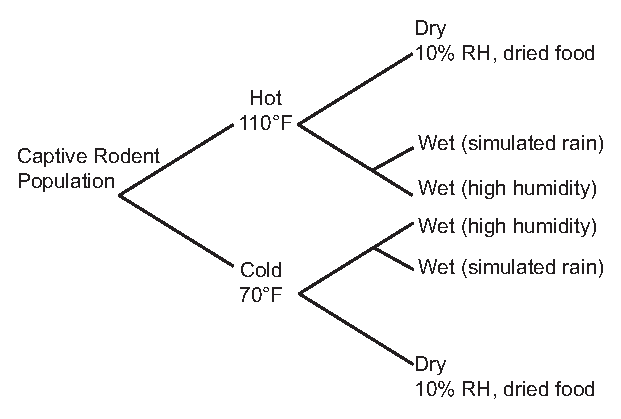
\includegraphics[width=1\textwidth]{exp_design_fig.eps}
  \end{center}
  %\hline
  \caption{\small{Animals are relegated into either hot or cold treatments. Within treatments (n=10 per treatment), animals are exposed to two weeks of varying levels of aridity, from simulated rainfall where water is available \textit{ad libitum}, to dry, where no water is available. RH=relative Humidity}}
\end{mdframed}
\end{wrapfigure}

Lastly, the genomic processes related to desert survival have yet to be characterized. The few studies of genetics that have been done have focused on the role of single members of the Aquaporin gene family (but see \cite{Bartolo:2007hy}), which are large membrane-bound proteins that are critically involved in renal water transport \citep{Kwon:2009bv,Verkman:2002ww,Brown:1995vo,Nielsen:1995cb}. These studies have shown that changes in Aquaporin (AQP) protein abundance and expression may be related to water availability \citep{Boselt:2009fb, Gallardo:2005fm,Bozinovic:2003eg}. In addition to changes in expression, another study showed that the AQP4 pathway was completely lost in the desert rodent \textit{Dipodomys merriami merriami} \citep{Huang:2001ti}. Despite these studies, we have a limited understanding of the genomics of renal water and solute regulation in desert animals. While AQPs are functionally important, water and solute balance is extraordinarily complex, and therefore single-gene studies are necessarily limited in their purview. A more complete understanding of this phenotype and its mechanistic underpinnings will require a sophisticated genome-level approach, which will be the outcome of the proposed research. 

\begin{center}
\textsc{{ii. Experimental Plan and Preliminary Results}} \\
\end{center}


\textbf{Specific Aim 1:} To fully understand the physiological effects of desert conditions on rodents, \ul{I will relate multiple physiological variables to differences in temperature, relative humidity, and water availability.} These experiments (and those described under Aim 2) are fundamentally linked to a series of environmental manipulations, described in \hyperlink{Figure 1}{Figure 1}. I hypothesize that, as a result of unique mechanisms related to solute and water balance, that average electrolyte concentrations will remain relatively constant throughout various experimental manipulations, but the variance in measured levels between individuals will increase in the most extreme conditions.


From all animals in experimental treatment groups (n=10 * 6 treatments=60 animals), I will collect a urine sample, and measure specific gravity and urine osmolality using an Atago UG-$\alpha$ urine refractometer. Serum electrolytes including potassium, sodium, BUN, creatinine, calcium and bicarbonate ion concentration will be measured, as will carbon dioxide production and oxygen consumption.

\textsc{{Preliminary Data:}} To date, I have generated a physiology dataset that consists of serum electrolytes and urine osmolality from 5 animals housed in the 'cold/simulated rain' treatment group. This small dataset allowed me to refine and perfect the protocols for data collection and analysis, and has already suggested interesting physiology. In the small subset of animals housed in the cool, wet, simulated rain conditions for a period of 3 weeks, all had serum Potassium levels \textgreater 8.0, Creatinine \textless 0.3, and Sodium \textgreater 151, which is significantly different than 'normal' levels in humans and other mammals.  

\textbf{Specific Aim 2:} \ul{I will understand the genetic response to extreme heat and aridity via a series of bisulfite sequencing and RNAseq experiments, and will link these patterns to individual physiologic state as defined in Aim 1.} Differences in renal methylation patterns and mRNA gene expression will be tested using the 10 individuals per treatment group (n=60 total, specified above). 

For analysis of the bisulfite sequence data, an accurate genome assembly is required. Using the existing draft genome (sequenced using startup funds) as a starting point, I will complete the genome assembly of the primary study organism, \textit{Peromyscus eremicus}. This process will be significantly aided by leveraging the existing genome sequence data available from several other \textit{Peromyscus} species. The genome will be validated by use of the CEGMA \citep{Parra:2007df} and REAPR \citep{Hunt:2013hj} algorithms. In general, this approach has been shown to be successful in producing high quality draft assemblies, though multiple assembly methods will be evaluated as per the findings of my previous work \citep{Bradnam:2013gx}.

For each  

\textsc{{Preliminary Data:}} To date, I have generated a RNAseq dataset that consists of approximately 30M 150nt SE Illumina reads from the same 5 animals housed in the 'cold/simulated rain' treatment group from which I collected physiology data. 

\begin{center}
\textsc{{iii. Budget Description}} \\
\end{center}

\textbf{Personnel:} The project described above requires significant personnel needs. PI MacManes is responsible for aspects this proposal. Specifically, he will oversee the design and execution of the genetic components of aim 1 and 2, which involves extraction of RNA from tissue samples, generation of mRNA sequencing libraries, sequencing on the Illumina HiSeq 2500 platform, and all bioinformatic analysis. MacManes will train the graduate student, and will interact with other project participants (undergraduate students). 2 months of summer salary per year is requested for all three years of the project. Salary is increased annually by 3\% to account for inflation, from a base rate of \$74000. In addition to the senior personnel, a PhD student and undergraduate student will be paid \$7000 and \$4500 respectively for 10 weeks of full time work on the proposed project. 

\textbf{Materials:} Direct costs will sum to approximately \$60000 per year. These costs will be used for, in approximate order of expense: Illumina RNA sequencing, Illumina DNA sequencing (for studies of methylation), Illumina sequencing library generation, general lab consumables, computer hardware upkeep, publications charges and general office supplies that directly related to the proposed project. 

\textbf{Indirect Costs and Fringe Benefits:} Facilities and Administration is charged at 47.5\% of MTDC based UNH’s federally negotiated rate. Fringe benefits for summer salaries are calculated at 7.7\% per UNH’s federally negotiated rates. 
 
\textbf{Total Project Costs:} Total project costs are expected to be approximately \$416,000 over 3 years.  

%\setcounter{page}{1}
%\thispagestyle{empty}
\singlespacing
\bibliographystyle{/Users/macmanes/Documents/army/pnas.bst}
\bibliography{/Users/macmanes/Documents/pero_transcriptome/biblio.bib}


































\end{document}
